\chapter{Language Usage Tutorial}

This will cover the configuration of the user's environment and the usage of Extend's features.

\section{Setup}
The Extend compiler requires that the OCaml Language and LLVM be installed on the host machine. Development was done in a virtual machine running the 64-bit Ubuntu operating system. In order to quickly get Extend up and running, please use \underline{\href{https://courseworks2.columbia.edu/courses/10787/files/673708/download}{this virtual machine}}, which has been provided as part of the course.

	\medskip \noindent After booting up the virtual machine, clone the Extend git repository:

	\begin{lstlisting}
		git clone https://github.com/ExtendLang/Extend.git
	\end{lstlisting}

\section{Compiling and Running Extend Code}
To build the Extend compiler, the first steps are the following.

	\begin{lstlisting}
cd Extend/
make
	\end{lstlisting}

	\medskip \noindent
	If this does not successfully build, run \texttt{eval `opam config env`}, which should configure the environment to use OPAM packages. Alternatively, add this command to your bash profile.

	 \medskip \noindent
	 After running \texttt{make}, you should see a \texttt{main.byte} file. To compile and run an Extend program, we have provided a shell script to simplify the process for the user:

	\begin{lstlisting}
	./compile.sh samples/helloworld.xtnd
	\end{lstlisting}

	\medskip \noindent
	This should produce an \texttt{out} file. Running \texttt{./out} should successfully execute the program.

\section{Writing Extend Code - The Basics}
As is tradition, here is "Hello World" in Extend. The following program, \texttt{helloworld.xtnd}, illustrates a basic usage of the Extend language.

\begin{lstlisting}
	main(args) {
	  return print_endline("Hello, World!");
	}
\end{lstlisting}

\medskip \noindent
Below is a short tour of the features of Extend. More detail can be found in the next chapter - the Language Reference Manual.

	\subsection{Adjusting to Extend's Declarative Nature}
	The biggest difference between Extend and most traditional programming languages is that the concept of an imperative statement does not exist. An Extend function consists solely of variable declarations, formula assignments, and a return expression. When a function is called, its \texttt{return} expression is evaluated, along with the values of any variables that the return expression depends on. In a traditional imperative language, the order of operations is determined explicitly by the developer; in Extend, the order is determined implicitly by the desired result.

	\medskip \noindent The following file compiles and prints successfully.

	\begin{lstlisting}
		main(args){
			foo := "Hello World!";     // Combined var declaration and formula assignment
			return print_endline(foo); // Return expression is a call to print_endline()
		}
	\end{lstlisting}

	\medskip \noindent The next file compiles, but might surprise you by not printing anything.

	\begin{lstlisting}
		main(args){
			foo := "Hello World!";     // Formula assigned, never evaluated
			bar := print_endline(foo); // Formula assigned, never evaluated
			return 0; 								 // Return expression is just 0
		}
	\end{lstlisting}
	\medskip \noindent And this file isn't a grammatical Extend program:

	\begin{lstlisting}
		main(args){
			foo := "Hello World!"; // OK
			print_endline(foo);    // Syntax error - not a declaration or assignment
			return foo;
		}
	\end{lstlisting}

	\medskip \noindent As illustrated, Extend only evaluates what is needed to produce the value required by \texttt{return}. Any non-essential declarations or formula assignments will not be evaluated by the program.

	\subsection{Functions}
	An Extend program is mostly composed of functions, declared with the usual syntax \texttt{f(x, y, ...)}. Each Extend program must have a main() function taking one argument, as shown above in "Hello World". Inside the function, this parameter will contain the command-line arguments. A function is composed of variable declarations and formula assignments and concludes with the \textbf{return} statement. It can return a value of any of the types discussed below, and it doesn't always need to return the same type.
	Note that the \textbf{return} statement is always the last statement in the function.

	\subsection{Data Types}
	Extend has three primitive data types: Number, String, and \texttt{empty}; and one composite type, Range. An example of each is shown below.

	\begin{lstlisting}
		myNumber    := 5;
		myString    := "Hello World";
		myEmpty     := empty;
		my2x3Range  := {3, 4, "five"; "a", "b", "c"};
	\end{lstlisting}

	\subsection{Variables}
	In Extend, \texttt{variables} are composed of cells to which formulas are assigned. The first time (and only the first time!) an individual cell is referenced by an expression, its value is calculated according to its assigned formula. A cell's value is not calculated if the cell is never referred to, and is never recalculated; all cell values are immutable. A cell's value can be any of Extend's types, and different cells of a single variable can have different types.

	\begin{lstlisting}
		[1,2] foo; // Declares a variable with 1 row and 2 columns (2 cells total)
		[1,3] bar := 4; // Declares a variable with 1 row and 3 columns and
		                // assigns the literal value 4 as the formula for each cell
		[1,2] baz;                 // Declares a 1x2 variable baz
		baz[0,0] = "first";   		 // Assigns literal "first" as the formula for the
		baz[0,1] = 1 + 1;          // 1st cell and the expression 1+1 for the 2nd cell
		life := 6, universe := 7;  // Declares 1x1 variables life and universe
		answer := life * universe; // Declares a 1x1 variable the_answer and assigns
															 // the formula life * universe to its sole cell
		[1,10] half_and_half;			 // Declares a 1x10 variable half_and_half
		half_and_half[0,0:5] = "milk";		// Assigns "milk" to the first five cells
		half_and_half[0,5:10] = "cream";  // and "cream" to the second five cells
	\end{lstlisting}

	\medskip \noindent
	\textbf{Note} that we declare a variable and assign a formula to all of its cells in a single line with \texttt{:=}. If the variable has already been declared, a formula must be assigned using \texttt{=} instead of \texttt{:=}. As illustrated in this example, a single formula can be assigned to multiple cells of a variable with the slice syntax. The converse is not true: multiple formulas applying to a single cell will cause a runtime error. The contents of the slice, as well as the dimensions of the variable, can be any expression that evaluates to a number, not just a literal number. For example, this code snippet assigns the dimensions based on the \texttt{howBig()} function and the "left" and "right" formulas based on the \texttt{breakpoint()} function:

	\begin{lstlisting}
		breakpoint() { return 7; }

		howBig() { return 11;	}

		foo_func() {
			[1,howBig()] foo;
			foo[0, :breakpoint()] = "left";
			foo[0, breakpoint():-1] = "right";
			foo[0, -1] = "last";
			return foo;
		}
	\end{lstlisting}

	\medskip \noindent
	This example also illustrates that the start (or end) index of a slice can be omitted if the developer wants the formula to apply from the beginning (or to the end) of the dimension, and that negative numbers can be used in a slice to count backwards from the end. The first time a variable is referred to (directly or indirectly) by the return expression, its dimensions and the formula assignment slices are computed; from that point on, they never change. A subtle point in the example above: the howBig() function is invoked once, but the breakpoint() function is actually called twice: once for the "left" formula, and once for the "right" formula.

		\subsubsection{Variables vs. Ranges - Similar, but not the same}
		A variable is not a data type; it is a collection of one or more cells with assigned formulas. A range is a value, which is internally implemented as a pointer to a subset of a variable's cells. A range is always composed of more than one value; a variable may have a single cell. The variable "backing" a range may not have been explicitly defined by the developer; for example, range literals are implemented using an anonymous variable.

	\subsection{Function Parameters - Using Dimensions}
		Function arguments can be signed with dimensions. You can use these in two different ways, depending on what your function is doing. As a convenient way to find out the size of a range argument, just give the dimensions names:

		\begin{lstlisting}
			foo([m,n] arg){
				return m * n; // m and n initialized through arg
			}
		\end{lstlisting}

		\medskip \noindent
		You can hardcode dimensions; if your function is called with a range whose dimensions don't match, a runtime error will occur:

		\begin{lstlisting}
			determinant([2,2] arg){
				return arg[0,0] * arg[1,1] - arg[0,1] * arg[1,0];
			}
		\end{lstlisting}
		\medskip \noindent
		You can also combine these two mechanisms, by repeating a variable name:
		\begin{lstlisting}
			betterBeSameSize([m,n] arg1, [m,n] arg2) {
				return "I guess they were the same size."; // Error if they were different
			}
		\end{lstlisting}

		\subsubsection{Enough theory. Show me a function that does something!}
		This function adds its two arguments.
		\begin{lstlisting}
			add(x, y) {
				return x + y;
			}
		\end{lstlisting}
		\medskip \noindent
		Come on, a real function.
		\begin{lstlisting}
			euclideanDistance([1,2] ptA, [1,2] ptB) {
				return sqrt((ptA[0] - ptB[0]) ** 2 + (ptA[1] - ptB[1]) ** 2);
			}
		\end{lstlisting}
		\medskip \noindent
		Tell me about that bit where you wrote ptA[0]!
		\subsubsection{Range Slicing \& Selection}
		The euclideanDistance() function above used a selection to extract the individual values from a range. ptA[0] is the first value of ptA and ptA[1] is the second value. Although ranges have rows and columns, you only need to give one index if a range is a vector---Extend will figure out what you mean. You can also get a slice, with essentially the same syntax as Python:
		\begin{lstlisting}
			addTheFirstThreeElements([1,n] some_vector) {
				return sum(some_vector[:3]);
			}
		\end{lstlisting}
		\medskip \noindent
		If you're dealing with a 2-D range, you can get a rectangle by slicing both the rows and the columns.
		\begin{lstlisting}
			topLeftCorner(m) {
				return m[:2,:2] // Returns a 2x2 range with m[0,0], m[0,1], m[1,0], m[1,1]
			}
		\end{lstlisting}
		\medskip \noindent
		\subsubsection{How is this like a spreadsheet?}
		Here's the Extend equivalent of this spreadsheet:
		\begin{center}
		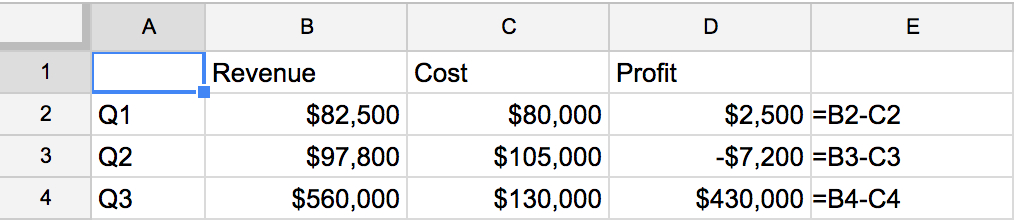
\includegraphics[width=7cm]{img/tutRCP.png}
		\end{center}
		\begin{lstlisting}
			calcProfit([n,1] revenue, [n,1] cost) {
				[n,1] profit := revenue[[0]] - cost[[0]];
				return profit;
			}
			main(args) {
				revenue := {82500; 97800; 560000};
				cost := {80000; 105000; 130000};
				profit := calcProfit(revenue, cost);
				return print_endline(profit);
			}
		\end{lstlisting}
		Writing revenue[[0]] and cost[[0]] instead of revenue[0] and cost[0] means that the nth cell of profit is calculated by subtracting the nth cells of cost from the nth cell of revenue; the number inside the brackets gets added to the row index of the left-hand-side cell. Here's how to calculate the change in profits from one quarter to the next:
		\begin{center}
		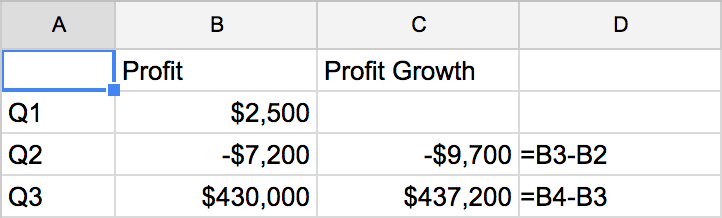
\includegraphics[width=7cm]{img/tutPG.png}
		\end{center}
		\begin{lstlisting}
			calcProfitGrowth([n,1] profits) {
				[n,1] profitGrowth := profits[[0]] - profits[[-1]];
				return profitGrowth;
			}
			main(args) {
				profits := {2500;-7200;430000};
				return print_endline(calcProfitGrowth(profits));
			}
		\end{lstlisting}

		\medskip \noindent
		Don't worry about the first cell - it'll be \texttt{empty}, not a program-ending \texttt{ArrayIndexOutOfBoundsException}. The selection syntax is very flexible; you can mix and match absolute and relative indexes and slices and omit the ones you don't need. There's a lot more examples in the language reference manual, but hopefully that should get you started! There's just one more special way you should know about to make a selection, since it's probably the most common selection you'll need.

		\subsubsection{The Hash Operator}
		The hash operator gets the cell that's in "the equivalent place" of the cell whose formula is being calculated. Here's the quick way to add two matrices:
		\begin{lstlisting}
			matrixAdd([m,n] arg1, [m,n] arg2) {
				[m,n] result := #arg1 + #arg2;
				return result;
			}
		\end{lstlisting}
		\medskip \noindent
		And here's one more example to show its flexibility, with the spreadsheet equivalent:
		\begin{center}
		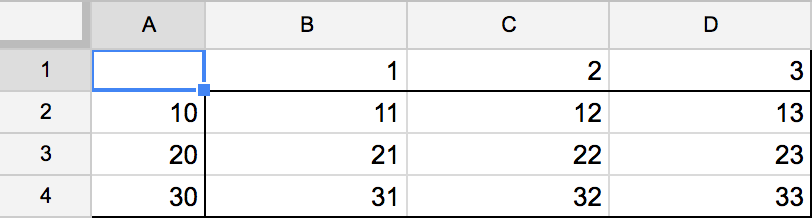
\includegraphics[width=7cm]{img/tutHash.png}
		\end{center}
		\begin{lstlisting}
			hashAdd([1,n] arg1, [m,1] arg2) {
				[m,n] result := #arg1 + #arg2;
				return result;
			}
		\end{lstlisting}
		\medskip \noindent
		If you call hashAdd with $\left\{1,2,3\right\}$ as the first argument and $\left\{10;20;30\right\}$ as the second argument, your result will be the matrix in the image. Enjoy making selections!

	\subsection{Cell Evaluation, Side Effects, and Precedence Expressions}
	It's time for a little more theory. As mentioned before, a cell's value is calculated at most once. It is evaluated when it is the only cell selected from a variable, or when a selection containing the cell is assigned as a range to another cell. In general, the language is designed so you don't have to think about this! However, if a cell formula calls a function with side effects, it's important to keep in mind that it will only be evaluated once for each cell with that formula.

	Another feature related to side effects is the precedence expression. If you want to call a function such as print\_endline() for its side effects, but don't want it to be your return statement, you can use a precedence expression (written with the \texttt{->} operator) to force the evaluation of one expression before another. For example, to display a prompt before asking the user for input, you could write:
	\begin{lstlisting}
	 	speed := print_endline("What is the air-speed velocity of an unladen swallow?")
								-> readline(STDIN);
	\end{lstlisting}
	A precedence expression calculates the first expression, discards the result, and evaluates to the second expression. Putting it all together, the following example should help clarify how cell evaluation is performed:

	\begin{lstlisting}
	main(args) {
		foo := print_endline("Once") -> 2;
		bar := foo + foo;
		return print_endline(bar);
	}
	\end{lstlisting}

	\medskip \noindent
	This program prints "Once" and then prints 4. Before calling print\_endline, Extend calculates the value of bar, which in turn requires the value of foo (twice). The first time foo's value is calculated, print\_endline() is called with the argument "Once", and then foo evaluates to the constant 2. The second time that foo's value is required to calculate bar, it's already available: it is 2. Therefore, print\_endline("Once") is not called a second time.

	\subsection{Operators}
	Extend includes a comprehensive set of operators. Each category is listed in order of precedence. A more detailed explanation of each operator can be found in the Language Reference Manual.

		\subsubsection{Arithmetic Operators}
			\begin{itemize}
				\item Unary Operations: \texttt{-}
				\item Binary Operations: \texttt{**, *, /, \%, +, -}
			\end{itemize}

		\subsubsection{Bitwise Operators}
			\begin{itemize}
				\item Unary Operations: \texttt{\~}
				\item Binary Operations: \texttt{<<, >>, \&, |, \^}
			\end{itemize}

		\subsubsection{Boolean Operators}
			\begin{itemize}
				\item Unary Operations: \texttt{!}
				\item Binary Operations: \texttt{==, !=, <, >, <=, >=, \&\&, ||}
			\end{itemize}

		\subsubsection{String Concatenation}
		Note that the \texttt{+} symbol can be used to perform concatenation between two strings.

		\begin{lstlisting}
			"Hello " + "World\n"
		\end{lstlisting}

		\subsubsection{The "Where am I?" operators}
		Extend has the \texttt{row()} and \texttt{column()} functions, which respectively return the row and column of the left-hand-side cell whose formula is being calculated.

		\subsubsection{The size and typeof operators}
		Extend offers a \texttt{typeof(expr)} operator, which takes an expression and returns Number, String, Range, or Empty (as a string). It also has the \texttt{size(expr)} operator, which returns the dimensions of its argument as a 1 x 2 range.


	\subsection{Conditionals}
	There are two types of conditional expressions: the if-then-else (ternary) conditional and a \texttt{switch} expression.

		\subsubsection{If-Then-Else}
		The two equivalent ways to write the ternary expression are as follows: \newline \newline
		C/Java style: \texttt{condition ? expr\_if\_true : expr\_if\_false} \newline
		Spreadsheet style: \texttt{if(conditional, expr\_if\_true, expr\_if\_false)} \newline \newline
		The predicate is always evaluated; only one of \texttt{expr\_if\_true} or \texttt{expr\_if\_false} will be evaluated---or neither, if the predicate is \texttt{empty}.


		\subsubsection{The Switch Expression}
		Below is an example of the switch expression used in a function:

		\begin{lstlisting}
			odd_or_even(foo){
				return switch(foo % 2) {
					case 0: "Even";
					case 1: "Odd";
					default: "Not an integer";
				};
			}
		\end{lstlisting}

	\medskip \noindent
	In the example above, the \texttt{switch} expression used \texttt{foo \% 2} as an argument; however, this is not required, so a switch expression can be used (as in Go) as a replacement for a sequence of if-then-else conditionals.

	\subsection{Import Statements}
	In Extend, you can import other Extend files at the top of your program via relative directory path. The use case is below:

	\begin{lstlisting}
		import "../programs/stat_library.xtnd"
	\end{lstlisting}

	\section{Illustrating the Benefits of Extend}
	Excel and Google Sheets are pretty easy to use. Why go to all this trouble? Spreadsheet applications require the use of manual input in order to apply the same calculation to a different set of data. Extend aims to tackle this problem by offering portability. Below is an example of a spreadsheet user calculating the unit vector of a column vector:

	\begin{center}
	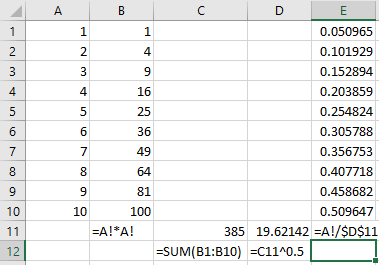
\includegraphics[width=7cm]{img/unitvector.png}
	\end{center}

	\medskip \noindent The Excel user must manually input the data, and additionally make space for the intermediate steps of the calculation. If the number of elements of the vector were changed, the formulas would need to be changed in the spreadsheet; similarly, if you needed to do this on a second vector, you would have to copy and paste the cells doing intermediate calculations. Below is the equivalent function in Extend, written to work on any column vector that is passed in:

	\begin{lstlisting}
		normalize_column_vector([m,1] arg) {
		  [m,1] squared_lengths := #arg * #arg, normalized := #arg / vector_norm;
		  vector_norm := sqrt(sum(squared_lengths));
		  return normalized;
		}
	\end{lstlisting}

	\medskip \noindent Another simple example is concatenating a row of strings of variable length with a common delimiter. This in an entirely manual operation for the spreadsheet user; a step-by-step attempt is shown below.

	\begin{center}
	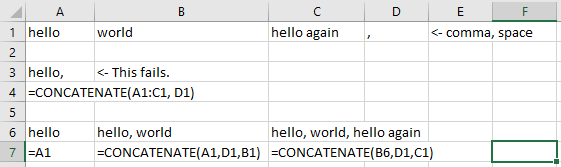
\includegraphics[width=9cm,height=3cm]{img/concatenation.png}
	\end{center}

	\medskip \noindent Performing a delimiter 'join' like the above can be performed in a simple program in Extend without knowing the size of the row. The following function, which is included in the Extend standard library, performs this on arguments of any size and can be reused throughout the program.

	\begin{lstlisting}
	main(args){
		bar := {"Hello", "Goodbye", "Hello Again"};
		str := ", ";
		return print_endline(concatRow(bar, str)); // prints "Hello, Goodbye, Hello Again"
	}

	concatRow([1,n] cells, joiner) {
	  [1,n] accum;
	  accum[0,0] = #cells;
	  accum[0,1:] = accum[[-1]] + joiner + #cells;
	  return accum[-1];
	}
	\end{lstlisting}

	\medskip \noindent As evidenced above by simple examples, Extend offers flexibility that is significantly harder to achieve with conventional spreadsheet applications. As the nature of the data grows in complexity and variety, Extend's value increases.

\section{Standard Library Functions}
Extend offers an assortment of standard library functions. The standard library is automatically imported into each Extend program.

\medskip \noindent
A complete listing of the functions in the standard library can be found in the Language Reference Manual; some of the more popular ones are listed below.
	\subsection{Basic Functions}
		\subsubsection{The toString() Function}
		The \texttt{toString()} function takes an argument and renders its value as a string.

		\begin{lstlisting}
			return "Hello " + toString(14); // "Hello 14"
		\end{lstlisting}

		\subsubsection{The Print Function}
		As used throughout this tutorial, the \texttt{print\_endline} function is used to print an expression with a newline.

		\subsubsection{Math Functions}
		Borrowing from C's standard library math functions, Extend offers: \texttt{sin, cos, tan, acos, asin, atan, sinh, cosh, tanh, exp, log, log10, sqrt, ceil, fabs} and \texttt{floor}.

		\begin{lstlisting}
			main(args){
				bar := sqrt(16);
				return print_endline(bar) -> 0; // Prints 4 to stdout
			}
		\end{lstlisting}

	\subsection{File I/O}
	Extend has \texttt{open, close, read, and write} functions to interact with files. Usage is as follows:

	\begin{lstlisting}
		main(args){
		  return write(STDOUT, read(open("test_file.txt", "r"),5)) -> 0; // Writes 5 characters from test_file.txt to stdout
		}
	\end{lstlisting}

	\subsection{Additional Standard Library Functions}

		\subsubsection{Flatten}
		The \texttt{flatten} function turns a rectangular range into a long row vector.

		\begin{lstlisting}
			flatten({1,2,3; 4,5,6}) // yields {1,2,3,4,5,6}
		\end{lstlisting}

		\subsubsection{Match}
		The \texttt{match} function takes a row or column vector and a value, and locates the index of that value, if applicable

		\subsubsection{Binary Search}
		The \texttt{bsearch} function will search a sorted column vector for a value.

		\subsubsection{Statistics Functions}
		Extend additionally offers basic statistical functions such as \texttt{sum, max, avg,} and \texttt{stddev}.

		\subsubsection{Matrix Multiplication}
		The \texttt{mmult} function multiples two compatible rectangular ranges together in matrix-fashion.

		\subsubsection{Concatenation}
		The \texttt{concatRow} function takes a column vector and a delimiter and returns a string of each element in the vector joined by the delimiter.

		\subsubsection{Repeat}
		The \texttt{repeat} function takes a string and number \texttt{x}, and returns a string where the argument string is repeated \texttt{x} times.
		\begin{lstlisting}
			repeat("Hello", 3) // "HelloHelloHello"
		\end{lstlisting}

		\subsubsection{Split \& Split to Range}
		The \texttt{split} function takes a string and a splitter and returns a vector of the delimited characters. Expanding on this, the \texttt{splittoRange} function takes a string, row splitter, and column splitter and returns a rectangular range with the characters delimited by the splitters.

		\subsubsection{Parsing Strings}
		The \texttt{parseString} function leverages the above two functions to create an actual range with the characters parsed as numeric values.

		\subsubsection{Reverse}
		Reverse takes a string and reverses it.

		\subsubsection{Trim Functions}
		The \texttt{trim} function removes preceding and following whitespace from a string and returns the new string. Similarly, the \texttt{ltrim} function removes preceding whitespace, and \texttt{rtrim} the following whitespace.

		\subsubsection{Plotting Bar Charts}
		Providing a file handle, a row vector, and an equivalently sized vector of labels to \texttt{bar\_chart} will allow the user to write a bar graph in GIF form to the file descriptor.
